\def\SPen#1{\varepsilon_{#1}}
\section{\label{sect:DERPAresults} Application to Gamow-Teller Response}
%\subsection{Computational framework}

%
% methods applied to GT response in Ca48
%
The Gamow-Teller charge-exchange operator is 
%
	\begin{eqnarray}
		\opO
	&=&
		\opO_- + \opO_+
	\nonumber \\
	&=&
		\sum_{k=1}^A
		\gvec{\sigma}(k) \tau_-(k)
	+
		\sum_{k=1}^A
		\gvec{\sigma}(k) \tau_+(k)
	\;,
	\label{eq:defGT}
	\end{eqnarray}
%
where $A$ is the number of nucleons, $\gvec{\sigma}$ is the spin tensor and $\tau_+$ 
($\tau_-$) is the isospin raising (lowering) operator.
The response function is for positive energies the response function of 
$\opO_-$ and is measured in the reaction 
$^{48}$Ca($p$,$n$)$^{48}$Sc at very forward angles. 
For negative energies the calculated 
function is $S_{\opO_+}$, which can be measured in the reaction
$^{48}$Ca($n$,$p$)$^{48}$K. 
Since the operator cannot change the spatial part of the particle wave 
functions, the ($n$,$p$) strength is zero when all orbits occupied by protons 
are also occupied by neutrons. In all calculations it is assumed that the 
proton and neutron orbits are identical (harmonic oscillator) wave functions.

\subsection{Computational Framework}
The same computational framework is used as in ref.~\cite{RGBA93}.
The single-particle state basis is chosen to consist of harmonic oscillator 
size parameter with size parameter $b=2.00$ fm. Note that the choice of the
 basis functions only affects the quantities
$\ME<\alpha|\opOhatless|\beta>$
of (\ref{eq:defS}).
As an effective interaction within this space a parameterization
\cite{Di83}
of a G-matrix deduced from a Bonn meson-exchange potential
\cite{HEA72}
is used. Such a G-matrix may
be considered as a realistic effective interaction within a space which is large
enough to incorporate collective long-range correlations, but too limited to
allow for the effect of short-range correlations to be
included~\cite{VDR91}.

For the single-particle energies $\SPen{\alpha}$ a spacing between major
shells of 16 MeV is adopted. Those
$\SPen{\alpha}$ which are close to the Fermi level are fixed in such a 
way
that energies of the states in adjacent odd nuclei with large spectroscopic
factors are reproduced when the Dyson equation (\ref{eq:Dyson}) is solved. 
This procedure
is discussed in more detail in
ref.~\cite{BRM91}.

The self-energy, used to solve the Dyson equation, is the so-called 
2p1h Tamm-Dancoff Approximation of ref.~\cite{RGBA93}. This self-energy
has been found to yield a good agreement with the 
spectral distributions measured in \eep\ reactions. A few typical 
distributions for shell model orbits are displayed in fig.~\ref{fig:gees}.
%%%%%%%%%%%%%%%%
%
% figures Gees
%
%%%%%%%%%%%%%%%%
\begin{figure}
\centerline{
\epsfig{figure=figures/tgif/gees.eps,width=11cm}
}
\caption[]{%
Representation of the single-particle propagator $g$ (\ref{eq:g1s}) for
three different proton shells, \viz\ a) $1s1/2$, b) $2s1/2$ and c) $1g9/2$.
The height of the peaks is the value of the $S_\alpha^{(p/h)}$ for the
fragment of which the position is given by the value of $E_\alpha^{(p/h)}$.
The vertical dotted lines denote the Fermi level at $-12$ MeV. Peaks to the
left of this line indicate the hole fragments ($\Sh{\alpha}$;$\Eh{\alpha}$)
while the others indicate the particle fragments
($\Sp{\alpha}$;$\Ep{\alpha}$).
In fig b) the main peak (quasi-particle peak) is reduced for plotting purposes,
the real height is $0.76$. The little arrows below the energy axis denote
the position of the poles of the single-pole propagator that is used in
RPA calculations. The strength of these poles equals one in the RPA case.
\label{fig:gees}}
\end{figure}
%%%%%%%%%%%%%%%%
This self-energy was found to give the best agreement with experiment.
Due to the energy-dependence of this self-energy the
particle and hole spectral strengths are fragmented and the calculated hole
spectral functions can be tested by comparison with those that are deduced
from \eep\ experiments%
\cite{HBJ88,BRM91,RAD92,WiH90,SBJ88,KBB89,SW91}.  

%\input{res_ERPA.tex}
\subsection{ERPA\label{sect:resultsEPRA}}
%
In the ERPA method of ref.~\cite{BAD90} some effects of the 
dressing of the single-particle 
propagators have been incorporated already. Firstly, the fragmentation due to
a second-order self-energy is taken into account  by the so-called 
self-screening diagrams, see fig.~\ref{fig:ERPAdiagrams}. 
These diagrams were included in the particle-hole interaction $\Gamma$. 
Secondly, if one solves the Dyson equation 
(\ref{eq:Dyson}) with a self-energy of second or higher order in the 
interaction $V$, one 
not only generates a large number of poles, but the main pole, with largest 
residue, is also shifted in energy relative to that of the single-pole 
propagator (\ref{eq:gHF}),
at least for the cases where one can 
speak about a distinguishable (quasi-particle) peak. In ERPA\cite{BAD90} 
the fact that
in principle all lines should be dressed is taken into account by 
using the shifted
energy in the expression for the single-pole propagator (\ref{eq:gHF}), 
which is
used to calculate the induced interaction. At the same time the HF energies are
used in the calculation of $L^0$ in (\ref{eq:ERPA}), because here the shifting
is supposed to be sufficiently included by the self-screening diagrams.

Before one focuses on an extended DRPA one should like to know what effects 
these features have. The self-screening appears to be essential, in the sense
that without it imaginary eigenvalues appear in the discrete calculation 
(or negative strength in the continuous calculation). The effect of using 
shifted poles in 
the calculation of the induced interaction is illustrated
in fig.~\ref{fig:plotENEN}. 
%%%%%%%%%%%%%%%
\begin{figure}
\centerline{
\epsfig{file=figures/gnuplot/plotENEN.ps,width=10cm}
}
\caption[]{
Comparison between the ERPA calculation as performed in \cite{BAD90} 
(solid line)
and the
same calculation, but with unmodified HF energies used everywhere (dashed line).
\label{fig:plotENEN}}
\end{figure}
%%%%%%%%%%%%%%%
Here the original ERPA calculation is compared with the same calculation, but 
with the original HF energies used also in the calculation of the induced 
interaction. 
%\input{res_DERPA.tex}
\subsection{DERPA}
%
As discussed already in section~\ref{sect:theoryDERPA},
%we are unable to incorporate the induced forces with  the fully fragmented 
%$L^f$ as used in DRPA, because the size of the matrices involved becomes
%prohibitive. 
the size of the matrices prohibits the use of the fully fragmented 
single-particle propagator, \cf\ fig.~\ref{fig:gees}.
Therefore, the approximation of a single-particle propagator 
$g^{3p}_\alpha$, an expression with only three terms is made for the
full propagator $g_\alpha$.
The following procedure is adopted. The main pole of $g_\alpha$ is taken 
to be the main pole of $g^{3p}_\alpha$ (\ie\ the energy, strength and 
width). All the remaining poles of $g_\alpha$ are, on each side of the Fermi 
energy, merged into a representative secondary pole (one above and one below the 
Fermi energy), with an energy equal to the strength weighted mean energy 
and a strength equal to the summed strength of the pole terms which they 
represent. These secondary poles are also given a width of $1.5$ MeV. 
By this approximation the problem of solving (\ref{eq:DERPA}) becomes 
feasible while the essential features, \ie\ the fragmentation of 
single-particle strength and partial occupation of the orbits, are preserved. 
So by comparing the results obtained with various approximations for the 
effective interaction $\Gamma$ one may still obtain a good impression of the 
importance of the inclusion of the induced forces in DRPA. This is the main 
purpose of the present study. If one aims  at a detailed description of the 
data, this approximation scheme may be too crude and also somewhat arbitrary. 
For orbits far away form the Fermi level there is not always a clearly 
distinguishable main peak, as is clear from fig.~\ref{fig:gees}.
Furthermore the combining of the poles with small strength into a 
few secondary 
poles induces an artificially large gap between the main poles and 
the secondary 
poles. A consequence of this is that also in the response, plotted 
in fig.~\ref{fig:DERPApn}, there is now an artificial gap between the main 
peaks and a bump at about $15$~MeV higher in energy. The latter is also 
an artifact of the adopted approximation scheme; it should be spread out over 
the whole energy range above the low-energy peaks.

%
%
% pn plot
%
%%%%%%%%%%%%%%%%%%
\begin{figure}
\centerline{
\epsfig{file=figures/gnuplot/pn_D_E_RPA.ps, width=10cm}
}
\caption[]{
Calculation of the Gamow-Teller ($p$,$n$) strength in $^{48}$Ca for 
the Dressed Independent Particle Approximation (DIPA), Dressed RPA (DRPA) and
Dressed Extended RPA (DERPA).
The single-particle propagator consists of only three poles. 
\label{fig:DERPApn}}
\end{figure}
%%%%%%%%%%%%%%%%%%
%
% np plot
%
%%%%%%%%%%%%%%%%%%
\begin{figure}
\centerline{
\epsfig{file=figures/gnuplot/np_D_E_RPA.ps, width=10cm}
}
\caption[]{
The Gamow-Teller ($n$,$p$) strength, see also fig.~\ref{fig:DERPApn}.
\label{fig:DERPAnp}}
\end{figure}
%%%%%%%%%%%%%%%%%%
%
Within this three-pole-approximation scheme for the $g_\alpha$ the effect 
of taking various approximations for $\Gamma$ is illustrated in 
figs.~\ref{fig:DERPApn} and \ref{fig:DERPAnp} for the Gamow-Teller 
($p$,$n$) and ($n$,$p$) strengths, respectively. In both cases one can 
observe that the 
induced interaction slightly enhances the (repulsive) effect of the bare 
interaction $V$ (here a G-matrix interaction). This is mainly discernible 
in the shift of relative strengths between the two lowest peaks in the 
($p$,$n$) 
strength. The integrated ($p$,$n$) strength up to $25$ MeV is only little 
affected by the induced forces and still matches the experimental value  
\cite{RGBA93}.
The calculated total integrated strengths for both the ($p$,$n$) and ($n$,$p$) 
reaction calculated with DERPA  agrees within one percent with the strength 
calculated using DRPA with the fully fragmented $L^f$ \cite{RGBA93}. 
